\documentclass[a4paper,12pt]{report} %размер бумаги устанавливаем А4, шрифт 12пунктов
\usepackage[utf8]{inputenc}
\usepackage[T2A]{fontenc}
\usepackage{geometry}
\usepackage{fancyhdr}
\usepackage{amsmath ,amsthm ,amssymb}
\usepackage{graphicx}
\usepackage{hyperref}
\usepackage{lipsum}
\usepackage{graphicx}
\usepackage{titlesec}
\usepackage{listingsutf8}
\renewcommand{\baselinestretch}{1.5} 
\usepackage[russian]{babel}
\setcounter{secnumdepth}{5}

\titleformat{\chapter}[block]
{\Large\bfseries}
{\thechapter.}{0.5em}{}

\usepackage{color}

\definecolor{lightgray}{rgb}{.9,.9,.9}
\definecolor{darkgray}{rgb}{.4,.4,.4}
\definecolor{purple}{rgb}{0.65, 0.12, 0.82}

\lstdefinelanguage{JavaScript}{
  keywords={typeof, new, true, false, catch, function, return, null, catch, switch, var, if, in, while, do, else, case, break},
  keywordstyle=\color{blue}\bfseries,
  ndkeywords={class, export, boolean, throw, implements, import, this},
  ndkeywordstyle=\color{darkgray}\bfseries,
  identifierstyle=\color{black},
  sensitive=false,
  comment=[l]{//},
  morecomment=[s]{/*}{*/},
  commentstyle=\color{purple}\ttfamily,
  stringstyle=\color{red}\ttfamily,
  morestring=[b]',
  morestring=[b]"
}

\lstset{
   language=JavaScript,
   backgroundcolor=\color{lightgray},
   extendedchars=true,
   basicstyle=\footnotesize\ttfamily,
   showstringspaces=false,
   showspaces=false,
   numbers=left,
   numberstyle=\footnotesize,
   numbersep=9pt,
   tabsize=2,
   breaklines=true,
   showtabs=false,
   captionpos=b
}

\usepackage{geometry} % Меняем поля страницы
\geometry{left=3cm}% левое поле
\geometry{right=2cm}% правое поле
\geometry{top=2cm}% верхнее поле
\geometry{bottom=2cm}% нижнее поле
\setlength{\parindent}{1.25cm}

\begin{document}
\begin{titlepage}
  \newpage

  \begin{center}
    ФЕДЕРАЛЬНОЕ АГЕНТСТВО ПО ОБРАЗОВАНИЮ РФ \\
    \vspace{1cm}
    Н-СКИЙ АРБУЗО-ЛИТЕЙНЫЙ ИНСТИТУТ \\*
    (ГОСУДАРСТВЕННЫЙ УНИВЕРСИТЕТ) \\*
    \hrulefill
  \end{center}

  \flushright{КАФЕДРА ХХХ}

  \vspace{8em}

  \begin{center}
    \Large Пояснительная записка \\ к дипломному проекту на тему:
  \end{center}

  \vspace{2.5em}

  \begin{center}
    \textsc{\textbf{исследование торсионных наногенераторов \linebreak стволовых клеток для борьбы с терроризмом}}
  \end{center}

  \vspace{6em}

  \begin{flushleft}
    Студент--дипломник \hrulefill Пупкин А.А. \\
    \vspace{1.5em}
    Научный руководитель \\
    доцент \hrulefill Иванов Б.Б.\\
    \vspace{1.5em}
    Рецензент \\
    к.ф.-м.н., в.н.с. АБВГ \hrulefill Петров В.В.\\
    \vspace{1.5em}
    Зав. кафедрой ХХХ \\
    д.ф-м.н, профессор \hrulefill Сидоров Г.Г.
  \end{flushleft}

  \vspace{\fill}

  \begin{center}
    Н-ск 2000
  \end{center}

\end{titlepage}% это титульный лист
\tableofcontents

\setlength{\parskip}{1em}
\chapter{Введение} %1 pages

Каждый день в мире взлетает и садится около 50 тысяч самолетов, среди
которых 30 тысяч - пасажирские, в воздухе одновременно их находятся около 10
тысяч. Кажется что для земного шара число достаточно маленькое, но если
посмотреть состояние в данный момент становится ясно что возушный траффик
сконтентирован в ограниченных областях.

Большинство самолетов - авиалинии - внутренние и внешние рейсы, следующие
примерно одними и теми же обозначенными маршрутами, и можно было бы просто
автоматизировать движение как железную дорогу, но помимо авиалиний в воздушном
пространстве так же могут быть и чартерные рейсы и военная авиация и метеозонды,
все это вносит большую долю неопределенности и непредсказуемости, особенно в
густонаселенных зонах - над одной лишь европой одновременно летят полторы тысячи
самолетов.

Возникает задача урегулирования воздушного траффика, которая на данный момент
решается тривиально - наземные станции наблюдения, связь диспетчер-пилот,
бортовые радары. Однако это все решения достаточно разрознены и требуют
формирования понимания ситуации на уровне человеческого восприятия или же некого
аппаратно-програмного обеспечения.

Наиболее прогрессивной является идея постороения сети на базе цифровой связи
самолет - самолет и самолет - наземная станция, в которой каждый узел может
передать и получить информацию о ближайшем возушном пространстве.
\newpage
\chapter{Современные проблемы авионики и автоматическое зависимое
  наблюдение-вещание} %8 pages

С развитием индустрии водушного транспорта - гражданская, космическая авиация,
самолето- и вертолётостроение - всё больше и больше возникает вопрос разработки
радиоэлектронной аппаратуры к воздушным судам. Требования к аппаратуре постоянно
растут - изначально от нее требовалось показывать пилотам информацию о положении
судна в воздухе, поддерживать курс и высоту (автопилот), обеспечивать связь с
диспетчером и экипажем, теперь же к требованиям добавляются диагностика лётных
агрегатов (двигатели, рулевые агрегаты, прочее), поддержание жизнеобеспечения
экипажа и пассажиров, радиолокация, информация о гео-положении
(GPS), внутренняя и внешняя видеорегистрация, и так далее. Технологический
прогресс ведет если не к полной автоматизации управлением суда, то как минимум к
его упрощению для человека.

\section{Основные проблемы}

\subsection{Внутренняя}
Внутренняя заключается в том что с ростом требований к бортовой аппаратуре
становится все сложнее добавить новый функционал к старому ``железу'', затраты
на разработку программного обеспечения к ней так же растут. Проблема решается
разделением системы на модули, каждый из которых выполняет определенную для него
функцию, от получения данных до управления другими системами. Вместе все модули
формируют БРЭО - Бортовое Радиоэлектронное Оборудование. Разделение на модули
так же уменьшает стоимость разработки ПО - какие то модули можно купить готовыми
с уже написанным и рабочим ПО, использовать их в своей системе и разработать
только недостающие/желаемые модули

\subsection{Внешняя}
Внешняя проблема - проблема взаимодействия судов и наземных объектов. В воздухе
летает огромное разнообразие самолетов и вертолетов, самых разнообразных стран
производства и годов выпуска, разных назначений. Это приводит к тому что
какой-то борт может ``глушить'' все остальные из-за того что он использует
частоты какого-то старого стандарта или же это намеренное глушение какого-то
военного самолета. Некоторые самолеты современные и могут общаться друг с другом
по радиосвязи и обмениваться данными, некоторые могут, но более старому
протоколу, не совместимому с современным. У какого-то борта может быть
неисправен радар, и так далее.

Казалось бы - можно решить проблему совместимостей просто добавив еще
соотвествующих модулей, но, к сожалению, это приведет к излишней (возможно даже
``зашкаливающей'') сложности/запутанности БРЭО, а так же, вероятно, к лишнему
весу судна - например установка дополнительных антенн.

В данной работе я рассматриваю одну из функций БРЭО - автоматическое зависимое
наблюдение-вещание (АЗНВ), на английском - ADS-B (Automated dependent
survelliance-broadcast). 

\section{Что такое АЗНВ}
АЗНВ - технология позволяющая пилотам и диспетчерам с высокой точностью получать
информацию о состоянии воздушного пространства - траффик, погодные условия,
аэронавигационная информация - в определенном радиусе ``вокруг себя''.
Абстрактно принцип работы - каждый борт вещает на определенной частоте иноформацию о себе и
слушает на определенной (возможно другой) частоте если передает ли какой другой
борт или наземная станция какую-то подобную информацию. Приемо-передатчик
передает эту информацию в другой модуль, который формирует ``картину мира''
вокруг себя и отрисовывает её на дисплее, возможно что отрисовкой занимается
другой модуль или ПО.

Система АЗНВ зависит от двух компонентов БРЭО - системы навигации (GPS, ГЛОНАСС)
и системы цифровой связи (data-link), в качестве последнего часто используют
модфицированный радар вторичного наблюдения (SSE, Secondary Survelliance Radar)
Mode S, работающий на частотах 978МГц или 1090МГц. В данной же работе
используется транспондер VDL Mode 4 (VHF Data-link, Очень высокочастная цифровая
связь режим 4, в дальшейшем - VDL-4).
\newpage
\chapter{А-Сеть и её реализация на основе стандарта\newline VDL-4} %8 pages

\section{Концепция А-Сети}
Возможность цифровой связи между судами в воздухе и наземными станциями
наталкивает на идею формирования на их базе самоорганизующейся ad-hoc сети. В
такой сети каждый узел может получить информацию с любого другого узла, даже вне
радиуса действия своей радиоаппаратуры. Такая сеть не требует центрального узла
который бы поддерживал и контролировал сеть или её участок. Реализация этой
концепции - А-Сеть на основе стандарта VDL-4.

\section{Требования А-Сети}
А-Сеть, очевидно, требует установленного на объекте транспондера VDL-4, но
помимо него требуется так же дополнительное оборудование, реализующее следующие
функции:
\begin{itemize}
\item измерение времени распространения сигнала от источника;
\item поддержка протоколов взаимодействия между объектами;
\item хранение текущего образа сети и его обновление;
\item формирование, хранение, доставку, поиск объекта назначения, маршрутизацию,
 коммутацию, контроль факта доставки и целостности пакета, включая пакеты
 передачи речи в цифровой форме;
\item вычисление расстояния между объектами по их координатным данным и времени
  распространения сигнала;
\end{itemize}

Каждый из объектов должен иметь свой уникальный адрес в сети, например можно
использовать уникальный номер в сети ATN.

Наземные и надводные неподвижные объекты с целью повышения точности определения
координат, корректирующего оборудования и контроля корректности в условиях
неуверенной работы глобальных систем спутниковой навигации (ГССН) (например, при
возбужденном состоянии ионосферы) могут быть привязаны:
\begin{itemize}
\item к географическим координатам (географическая привязка);
\item к задающему генератору Сети и/или UTC SU (временная привязка);
\item к сети ATN (сетевая привязка).
\end{itemize}
Последний вид привязки может быть использован для расширения зоны доступа
Сети к аэродромам, радиолокационным станциям, диспетчерским службам, станциям
слежения и т.п.

Географически привязанные объекты должны устанавливаться на отдельных
геодезических постаментах для снижения погрешностей, связанных с сезонными
колебаниями грунта. Конструкция их антенн должна обеспечивать необходимую
защищенность от эффектов многолучевого распространения и затенения со стороны
препятствий.

Сетевые адреса (номера) объектов, имеющих географическую, временную и сетевую
привязки, должны быть известны всем объектам сети, помимо этого рекомендуется
использовать системы глобальной навигации разных стандартов для повышения
точности.

\section{Возможнсти предостовляемые А-Сетью}

\begin{itemize}
\item Точность - При наличии в сети четырех и более объектов возможно
  определение реальных координат их всех, а так же и внешних объектов. 
\item Маштабируемость - возможность расширения зоны налюблюдения в пределах
  доступа сети.
\item Надежность - возможность маршрутизации ``в обход'' позволяет сохранить
  соединение при возникновении помехи. Разлом в сети не выводит её из строя -
  каждый фрагмент сохраняет способность автономного функционирования.
\item Защищенность - наличие расчета расстояния до объекта (и последующее
  вычисление реальных координат) позволяет исключать из образа сети ложные
  объекты.
\item Поиск по сети - при необходимости передать сообщение конкретному объекту
  может быть использован принцип ``штурма'' - широковещательная рассылка запроса
  на соединение с защитой от повторной передачи по одному и тому же участку
\item Приоритезация - Наличие образа в Сети на объекте дает возможность
  обеспечить ``ручную'' маршрутизацию сообщения или автоматическую в
  соответствие с его рангом. Срочное сообщение следует маршрутизировать с
  позиции минимального количества переприемов,  вносящих основную задержку.
  Сообщение, требующее повышенной степени достоверности передачи, следует
  маршрутизировать через максимально короткие радиоканалы, обладающие (в
  статистике) лучшей помехоустойчивостью. Маршруты сообщений, не требующих
  специального внимания, должны минимизировать относительные потери пропускной
  способности на ребрах сети. 
\item Голосовая связь - в случае экстренной ситуации или при невозможности
  прямого радиодоступа есть возожмность установить речевую связь.
\end{itemize}
\newpage

\chapter{Разработка функциональной схемы транспондера и технических требований к
  системе индикации} %8 pages 
\section{Трансподнер VDL-4}
\begin{figure}[!ht]
  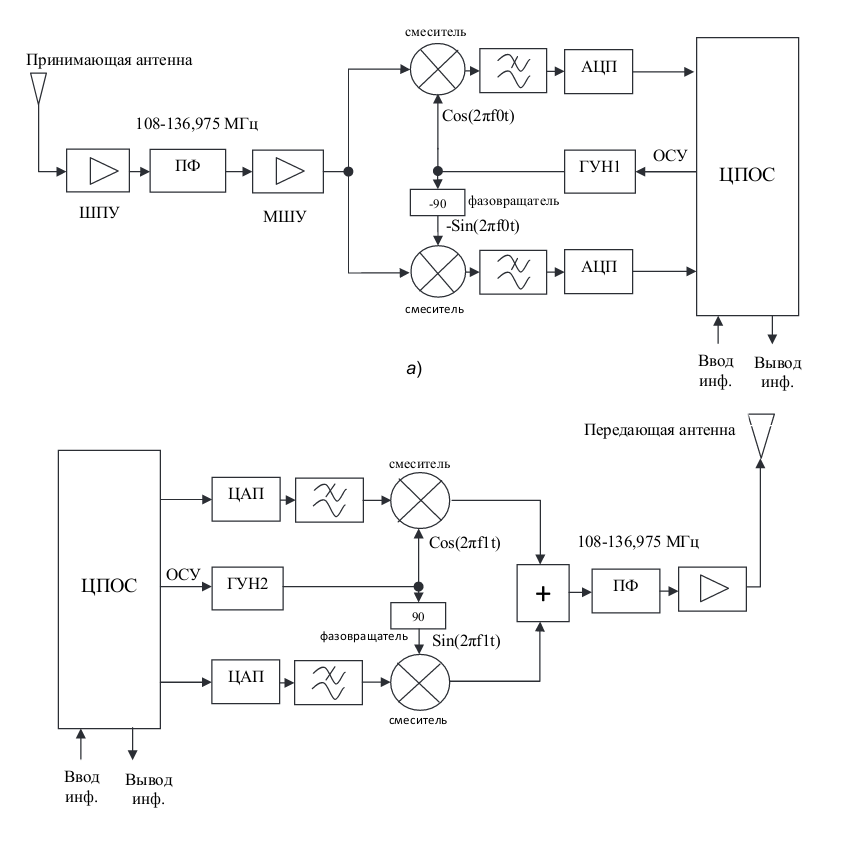
\includegraphics[width=0.9\textwidth]{vdl4}
  \caption{функциональная схема транспондера VDL-4}
\end{figure}

\begin{itemize}
\item [ЦПОС] Центральный процессор обработки сигналов
\item [МШУ] Малошумящий усилитель
\item [ГУН] Генератор управляемый напряжением
\item [ПФ] Полосовой фильтр
\item [АЦП] Аналогово-цифвровой преобразователь
\item [ЦАП] Цифро-аналоговый преобразователь
\end{itemize}
\newpage

\section{Система индикации}
Система индикации будет получать данные от транспондера в виде сформированного
текстового файла, возможна реализация тестового режима в котором будут показаные
тестовые (не соотвествующие действительности) объекты сети, с целью проверки
работоспособности системы индикации как таковой.

\subsection{Основные требования}
Система индикации должна:
\begin{itemize}
\item Показывать текущее положение объекта на котором установлена данная система
  (себя)
\item Показывать радиус действия прямого радиодоступа - 400км
\item Показывать другие объекты сети:
  \begin{itemize}
  \item Самолеты, находящиеся в радиусе прямого радиодоступа
  \item Самолеты, находящиеся в зоне действия сети (при запросе расширения зоны
    наблюдения)
  \item Наземные и водные станции
  \end{itemize}
\item Планируемый курс определенного объекта (по запросу)
\end{itemize}

Для тестового режима, реализуемого в данной работе реализуем следующий
функционал:
\begin{itemize}
\item Показываем себя - самолет летящий с фиксированным курсом и скоростью из
  начальных координат г. Москвы.
\item 2-3 самолета, летящих недалеко от нас с фиксированными курсами и
  скоростями.
\item Самолеты, покинувшие область прямого радиодоступа будут помечаться как
  самолеты ``в сети'' пока расстояние до них не станет больше 800км, после чего
  они полностью исчезнут с карты, до тех пор пока мы не встретимся с ними снова.
\end{itemize}

\subsection{Тенические требования}
Система индикации должна работать на основных платформах: Microsoft\copyright
Windows\copyright, Mac OS X, Linux с системой окон X11. Так же желательна
поддержка мобильных систем Android и Apple iOS.
\newpage

\chapter{Разработка прикладного алгоритмического и \newline програмного
  обеспения  системы индикации} %8 pages 
\section{Выбор платформы}
Для поддержания наибольшего числа платформ и легкости разработки, поддержки и
разработки системы индикации, я решил использовать платформу HTML5. Система
индикации (в дальшейшем СИ) написана на языке JavaScript с использованием
нескольких сторонних библиотек.

\subsection{Особенности платформы}
СИ может быть запущена из практически любого современного браузера - IE11,
Firefox, Chrome, Safari, но в целях удобства и потенциальной возможности доступа
к аппаратной части я использовал оболочку Electron - окружение позволяющее
написать приложение целиком на JavaScript\\HTML5 и при этом иметь функционал
``родного'' приложения - доступ к файловой системе, внешним устройствам,
функционалу конкретной операционной системе (уведомления, интеграция).

\subsection{Используемые технологии}
СИ в большей части использует библиотеку обработки и отображения данных - d3.js.
Данная библиотека позволяет, на основании входных данных выполнять определенные
действия - создавать, изменять, удалять указанные узлы. В данной работе при
помощи этой библиотеки управляется SVG элементы, строящие векторное
представление ортографической проекции земного шара (границы суши и земли) и
объектов нахоящихся на нём. Библиотека так же позволяет напрямую использовать
координаты в формате широта-долгота.

\subsection{Алгоритим программы}
Алгоритм программы заключается в следующем:
\begin{itemize}
\item Получить данные от транспондера (или сформировать их для тестового режима)
\item Нормализовать данные, обновить внутренний образ сети на их основе (в
  тестовом режиме данные обновляются за счет предыдущего состояния)
\item Передать данные о координатах в объекты d3.js
\item Модифицировать объекты d3.js для отображения дополнительной информации
  (направление, бортовой номер, скорость, тип)
\item Повторить все шаги снова по прохождении интервала обновления
\end{itemize}
\newpage

Исходный код программы:

\lstinputlisting[caption=client/index.js]{../client/index.js}
\lstinputlisting[caption=app.js]{../app.js}
\lstinputlisting[caption=index.html]{../index.html}

\newpage
\chapter{Разработка вопросов по экологии и безопасности жизнидеятельности при
  работе с электронной \newline аппаратурой} %8 pages
\section{Условия труда при работе с электронной аппаратурой}
При работе с электронной аппаратурой, в частности с комьютерами типа IBM PC,
человек подвергается различными вредными воздействиями: электро-магнитное
излучение, в частости от экрана монитора, шум системы охлажения, мерцание
экрана, статическое электричество.

Использование пилотами аппаратуры так же накладывает дополнительные требования:
аппаратура не должна отвлекать пилота от работы шумом или мерцанием,
использование аппаратуры не должно вызывать дискомфорта - надписи должны быть
легкочитаемы, интерфейс и схемы - разборчивы - пилот не должен прикладывать
дополнительные усилия, не должен вглядываться в дисплей чтобы получить
информацю.
\section{Анализ основных вредных факторов}
\subsection{Уровень шума}
Шумы обладают несколькими раздражающими факторами: они монотонны по свой природе
- повторяющиеся механические взаимодействия, деформации, вибрации, и при этом
изменчивы с течением времени - накапливается пыль из-за которой возникают
дополнительные вибрации, смазка подвижных деталей приходит в негодность, система
охлажения изменяет свою интенсивность в соответсвии с нагрузкой.

Под воздействием шумов человек раздражается, часто обращает внимание на источник
шума или пытается его определить, помимо этого в целом падает внимание,
увеличивается задерка реакции, увеличивается вероятность совершения ошибки
человеком.

В столь ответсвенной деятельности как пилотирование самолета или управление
полетами с земли подобные негативные факторы недопустимы и должны быть сведены к
минимуму.накапливается пыль из-за которой возникают дополнительные вибрации,
смазка подвижных деталей приходит в негодность, система охлажения изменяет свою
интенсивность в соответсвии с нагрузкой.

Под воздействием шумов человек раздражается, часто обращает внимание на источник
шума или пытается его определить, помимо этого в целом падает внимание,
увеличивается задерка реакции, увеличивается вероятность совершения ошибки
человеком.

В столь ответсвенной деятельности как пилотирование самолета или управление
полетами с земли подобные негативные факторы недопустимы и должны быть сведены к
минимуму.
\subsection{Электромагнитное излучение}
Дисплей монитора, будь то ЭЛТ или ЖК является основным иточником вредного
воздействия на человека. ЭЛТ мониторы, несомненно куда гораздо больше наносят
вреда нежели ЖК, но на данный момент они практически вышли из эксплуатации
повсеместно и встретить их можно только на очень старых ПК, которые не
обновлялись уже несколько поколений
\newpage
\chapter{Технико-экономическеой обоснование. Сравнение системы индиации с
  аналогами с помощью метода анализа иерархий} %8 pages
\lipsum [1]
\newpage
\chapter{Заключение}
\end{document}